\documentclass[]{article}

\usepackage[a4paper, total={6in, 9in}]{geometry}
\usepackage{authblk}
\usepackage{hyperref}
\usepackage{listings}
\usepackage{graphicx}
\usepackage[export]{adjustbox}
\usepackage{subfig}
\usepackage{float}
\usepackage{amsmath,amsfonts}
\usepackage{mathpazo}
\usepackage{amsmath}
\usepackage{graphicx}
\usepackage{calrsfs}
\usepackage{fancyvrb}
\usepackage{tikz}
\renewcommand*\contentsname{Table Of Contents}
%opening
\title{\textbf{\huge Computational Physics}}
\author[1]{ Vinit P. Doke}
\affil[1]{{
		Department of Physics\\ 
		Indian Institute of Technology\\
		Powai, Mumbai 400076 \\
		{Email:} \texttt{vinitdoke@gmail.com , 190260018@iitb.ac.in
		}.}
}
\date{{ Mentor: Chaitanya Kumar }}
\pagestyle{headings}
\hypersetup{
	colorlinks=true,
	linkcolor=blue,
	filecolor=blue,      
	urlcolor=blue,
}



\begin{document}


\maketitle


\begin{figure}[h]
	
	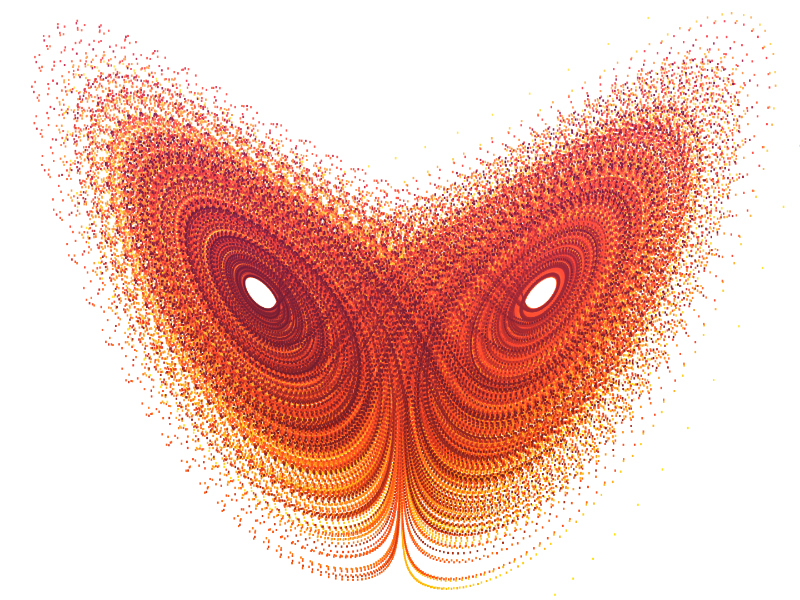
\includegraphics[width=1.1\linewidth]{lorenzattractor}
	\caption{Lorrenz Attractor}
	\label{fig:waveinterference}
\end{figure}

\newpage
\tableofcontents
%\newpage
\listoffigures


\newpage
\section{Introduction}
	\par With greater strides being made in Experimental Physics, we are witnessing data volumes that were never seen before. For instance, the \href{https://home.cern/news/news/computing/cern-data-centre-passes-200-petabyte-milestone}{Large Hadron Collider generates petabytes of data per second.} This warrants the use of computers to analyse, reformat and simulate various tasks in Physics. This is the field of study represented by Computational Sciences, Computational Physics being the application in Physics.\medskip
	\par Most numerical calculations in physics fall into one of several general categories, based on the mathematical operations that their solution requires. Examples of common operations include calculation of integrals and derivatives, linear algebra tasks such as matrix inversion or the calculation of eigenvalues, and the solution of differential equations, including both ordinary and partial differential equations. 
     If we know how to perform each of the basic operation types then we can solve most problems we are likely to encounter as physicists. I shall study individually the computational techniques used to perform various operations and then apply the solution to wide range of physics problems.
\subsection{Using Python}
Being an interpreted language, Python provides a much more natural coding experience. The plethora of support libraries available for it make it an ideal choice for scientific computing purposes. Some of the libraries required for this project include \textbf{Numpy, Pandas, Matplotlib, VPython, SciPy} etc. 
	\par Though many of these libraries provide in-built functionalities for carrying out various numerical operations, we shall follow a ground up approach towards these operations, exploring the methods followed to port them to a computer.
\subsection{Numerical Methods}
We shall see various methods of numerical evaluations of maths operations and then deal with the ways of calculating the errors produced due to either approximations or precision value errors (inherent to Python due to way the data types are stored). I shall be simultaneously solving problems pertaining to varied areas of Physics related to the mathematical methods which are linked here as follows:
 
\begin{enumerate}
	\item \hyperlink{section.2}{Data Visualisation}
	\item \hyperlink{section.3}{Integration}
	\item \hyperlink{section.4}{Solutions Of Non-Linear Equations}
	\item \hyperlink{section.5}{Ordinary Differential Equations}
	
	\item \hyperlink{section.6}{Random Processes}
	\item \hyperlink{section.6}{Monte-Carlo Methods}
	
	%\item Linear Equations
	%\item Non-Linear Equations
\end{enumerate}
\newpage
\section{Data Visualisation}
To make sense of the vast amounts of data, to study trends, patterns and various other characteristics, Visualisation serves as an indispensable tool. Data Viz. in itself is another vast domain of study, yet it has its uses in Physics. Graphs are fundamental in Physics followed by images and animations. Here, I deal with \textbf{Graphs, Density Plots, Scatter Plots and Images}.
\subsection{Graphs}
2D Graphs require datasets of points to be represented on a coordinate plane. One often encounters such datasets in Physics, having data regarding a dependent variable changing with an independent one. However, to plot functions, we need to evaluate them at a linear space of points between the required range to produce illusion of continuity. The computer draws straight-lines between the points. So the end-result is not smooth but a set of line-segments. However, sampling the functions at hundreds of such points enables the creation of smooth-looking curves.\medskip \\
\par The underlying code plots functions of form $r=f(\theta)$, i.e. explicit in $r$ and $\theta$.
\\
\\ \\
\begin{lstlisting}[language=Python, caption=Polar Plot, frame=single ]
import numpy as np
import matplotlib.pyplot as plt
%matplotlib qt5 #for jupyter notebooks only


thetas=np.linspace(#range of theta, #number of sample points) 
def cart(theta, r):
	x=r*np.cos(theta)
	y=r*np.sin(theta)
	return (x,y)
def func(theta):
	return #function here

X=[]
Y=[]
for theta in thetas:
	x,y=cart(theta, func(theta))
	X.append(x)
	Y.append(y)
plt.plot(Y,X, 'b')
plt.xlabel('X')
plt.ylabel('Y')
plt.title(# Function Name)
\end{lstlisting}
\begin{figure}[H]
	\centering
	\subfloat[$f(\theta)=e^{\cos \theta}-2\cos4\theta+\sin^{5} \dfrac{\theta}{12} $]{{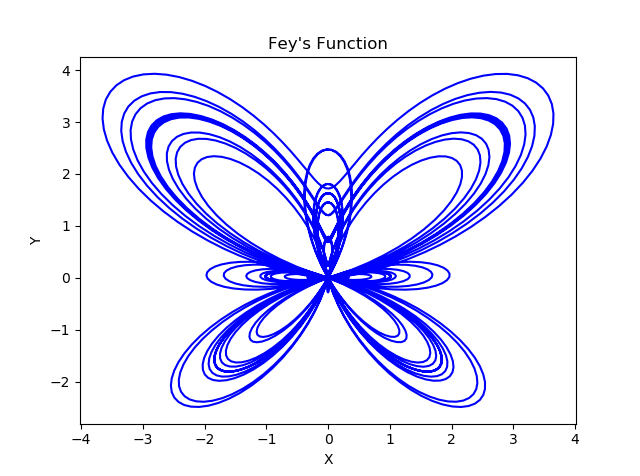
\includegraphics[width=7cm]{FeyFunc} }}%
	%\qquad
	\subfloat[$f(\theta)=\theta^{2}$]{{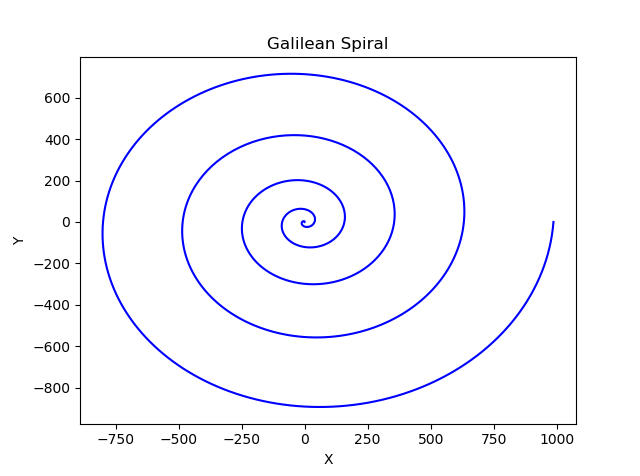
\includegraphics[width=7cm]{GalileanSpiral} }}%
	\caption{Polar Plots}%
	\label{fig:example}%
\end{figure}
\subsection{Density Plots and Images}
A \textbf{Density Plot} uses colours or brightness to represent magnitude on a 2D-Grid. In Python, we can pass an array of data, which can be 3D too. In this case, the values are interpreted as RGB values for each pixel in the grid. Consequently, many image formats are imported to Python in \textbf{3D-\textit{arrays}}. For instance, \textbf{FITS} (Flexible Image Transport System) is a widely used data format for storing astronomical observations by telescopes.\\
\par The underlying code displays the wave interference pattern for 2 plane waves produced in a medium at a particular separation.
\begin{lstlisting}[language=Python, caption=Interfernce Pattern, frame=single, label={lst:L2} ]
amp=1
wavelength=5
d=20
k=2*np.pi/wavelength
pond=np.zeros((500,500)) # two waves in a 1m*1m pond on a 500*500 grid
def dist(p1,p2):
	x1,y1=p1
	x2,y2=p2
	x1=conv_units(x1)
	x2=conv_units(x2)
	y1=conv_units(y1)
	y2=conv_units(y2)
	return ((x2-x1)**2+(y2-y1)**2)**(0.5)
def height1(p):
	return amp*np.sin(k*dist(p1,p))
def height2(p):
	return amp*np.sin(k*dist(p2,p))
def conv_units(point):
	return point/5
def conv_units2(point):
	return point*5
def height(p):
	return height1(p)+height2(p)
p1=(250,200)
p2=(250,200+conv_units2(20))
for i in range(500):
	for j in range(500):
		pond[i][j]=height((i,j))
pond=pond/2
plt.imshow(pond,interpolation='bicubic')
\end{lstlisting}
\begin{figure}[H]
	\centering
	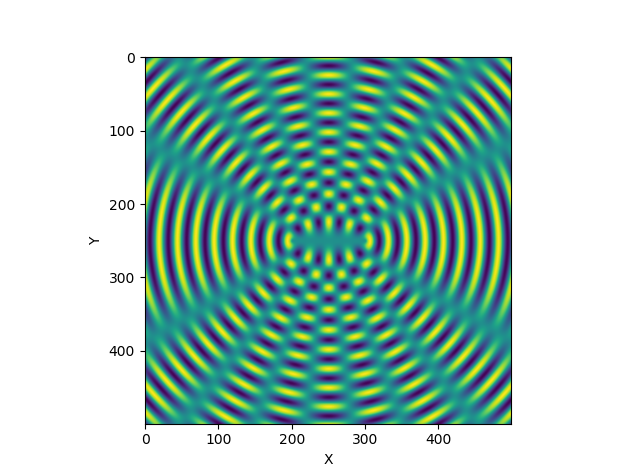
\includegraphics[width=0.7\linewidth]{WaveInterference}
	\caption{OUTPUT for Listing \ref{lst:L2}}
	\label{fig:waveinterference}
\end{figure}
\newpage
\section{Integration}
\label{sec:Int}
\subsection{Trapezoidal Rule}
We evaluate the integral for $f(x)$ in range $(a,b)$. One way would be to divide the range into $N$ slices like rectangles or trapezoids. As the name suggests, we approximate the function between $x_{i}$ and $x_{i+1}$ slices as a trapezium of $l1=f(x_{i})$ and $l2=f(x_{i+1})$ with separation  $h=(b-a)/N$, which will be same for all the trapeziums. Let the true value of the Integral be represented by $I$. Then the approximated integral is represented by $I_{0}$, given by:
\[\begin{split}
I_{0}&=\sum_{i=1}^{N}\dfrac{h}{2}[f(a+(i-1)h))+f(a+ih)] \\
%&=\dfrac{h}{2}[f(a)+f(a+h)+f(a+h)+......f(b)]
&=\dfrac{h}{2}[f(a)+f(b)+2(f(a+h))....2f(a+(N-1)h)]\\
&= \dfrac{h}{2}[f(a)+f(b)+2\sum_{i=1}^{N-1}f(a+ih)]\\
&\approx I\\
\end{split}
\]
Naturally, we will have greater precision for higher values of N. Generally, we use Adaptive Integral Method (discussed \hyperref[subsec:3.4]{here}), to obtain results within the desired level of accuracy.
\begin{lstlisting}[language=Python, caption=Trapezoidal Rule, frame=single, label={lst:L3} ]
def f(x):
	return x**4-2*x+1 #Function here
N= #Number Of Divisions
a= #start range
b= #end range
h=(b-a)/N
integ=f(a)/2+f(b)/2
for i in range(1,N):
	integ+=f(a+i*h)
integ*=h
print(integ) #Final Solution
\end{lstlisting}
\subsection{Simpson's Rule}
In Trapezoidal Rule, we approximate the curve by trapeziums, however we could fit a higher-order polynomial to our sliced function for better accuracy. Simpson's Rule does exactly that with polynomials of degree 2, i.e. Quadratic Expressions. We divide the range of $f(x)$, $(a,b)$ into $N$ equally spaced slices of width $h=(b-a)/N$. Let us consider 3 points, $\{-h,0,h\}$. The Quadratic polynomial passing through these points would be:
 
\[	f(x)=ax^{2}+bx+c\]
\[	f(-h)=ah^{2}-bh+c\]
\[	f(0)=c\]
\[	f(h)=ah^{2}+bh+c\]
Solving for the coefficients gives us the constants $a,b,c$ in terms of $h$. Now, we integrate over the slice $[-h,h]$ as follows:
\[\int_{-h}^{h}(ax^{2}+bx+c)dx=\dfrac{h}{3}[f(-h)+4f(0)+f(h)]  \]
Performing this integral for all slices of form $x_{i-1},x_{i},x_{i+1}$ returns the general approximate integral $I_{0}$ as:
\[\begin{split}
I_{0}&=\dfrac{h}{3}[f(a)+f(b)+4\sum_{k=1}^{Odd}f(a+kh)+2\sum_{k=2}^{Even}f(a+kh)]\\
&\approx I
\end{split}\]
Due to better order approximation, Simpson's rule generally yields more accurate results than the Trapezoidal rule in lesser steps ($N$). To obtain results within a specified degree of accuracy, we use the Adaptive Integral Method for Simpson's Rule (discussed \hyperref[subsec:3.4]{here}).
\begin{lstlisting}[language=Python, caption=Simpson's Rule, frame=single, label={lst:L4} ]
def f(x):
	return x**4-2*x+1 #function here
a= #start range
b= #end range
N= #Number of Divisions
h=(b-a)/N
s=f(a)+f(b)
for i in range(1,N,2):
	s+=4*f(a+i*h)
for i in range(2,N-1,2):
	s+=2*f(a+i*h)
s=s*h/3 
print(s)#Final Value
\end{lstlisting}
\subsubsection{Diffraction Limit Of Telescope}
Our ability to resolve detail in astronomical observations is
limited by the diffraction of light in our telescopes.  Light from stars
can be treated effectively as coming from a point source at infinity.  When
such light, with wavelength~$\lambda$, passes through the circular aperture
of a telescope (which we'll assume to have unit radius) and is focused by
the telescope in the focal plane, it produces not a single dot, but a
circular diffraction pattern consisting of central spot surrounded by a
series of concentric rings.  The intensity of the light in this diffraction
pattern is given by
\begin{displaymath}
I(r) = \biggl( {J_1(kr)\over kr} \biggr)^2,
\end{displaymath}
where $r$ is the distance in the focal plane from the center of the
diffraction pattern, $k=2\pi/\lambda$, and $J_1(x)$ is a Bessel function.
The Bessel functions~$J_m(x)$ are given by
\begin{displaymath}
J_m(x) = {\dfrac{1}{\pi}} \int_0^\pi \cos(m\theta - x\sin\theta) \ d\theta
\end{displaymath}
where $m$ is a nonnegative integer and $x\ge0$. \\

Here, I work out the image of the focal plane for light of $\lambda=500 nm$
\begin{lstlisting}[language=Python, caption=Bessel Function, frame=single, label={lst:L5} ]
def J(m,x):
	def f(t):
		return np.cos(m*t-x*np.sin(t))
	a=0
	b=np.pi
	N=1000
	h=(b-a)/N
	s=f(a)+f(b)
	for i in range(1,N,2):
		s+=4*f(a+i*h)
	for j in range(2,N-1,2):
		s+=2*f(a+j*h)
	s*=h/3
	return (1/(np.pi)*s)
\end{lstlisting}
\begin{figure}[H]
	\centering
	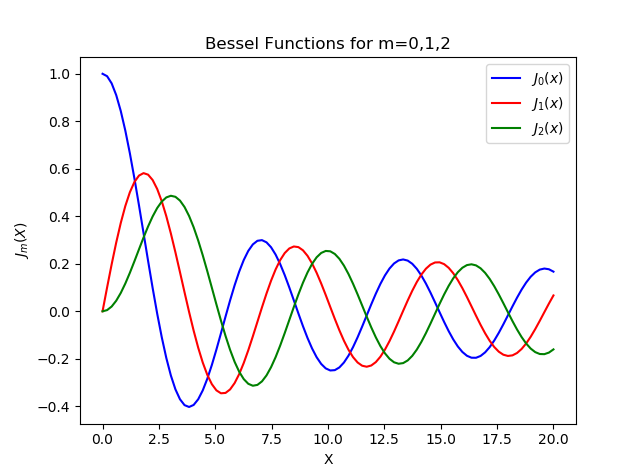
\includegraphics[width=0.7\linewidth]{BesselFunction}
	\caption{Plot of Bessel Functions}
	\label{fig:besselfunction}
\end{figure}

\begin{lstlisting}[language=Python, caption=Main Function, frame=single, label={lst:L6} ]
focal_plane=np.array([[0 for i in range(500)] for i in range(500)])
center=(250,250)
wavelength=62.5
k=2*np.pi/wavelength
def dist(point):
	x0,y0=center
	x,y=point
	return np.sqrt((x0-x)**2+(y0-y)**2)  
def I(r):
	return ((J(1,k*r))/(k*r))**2
for i in range(500):
	for j in range(500):
		focal_plane[i][j]=dist((i,j))
fp2=I(focal_plane)
mean=fp2.mean()
std=fp2.std()
plt.imshow(fp2,'cividis' ,vmax=mean+0.5*std, interpolation='bicubic')
\end{lstlisting}
\newpage
\begin{figure}[H]
	\centering
	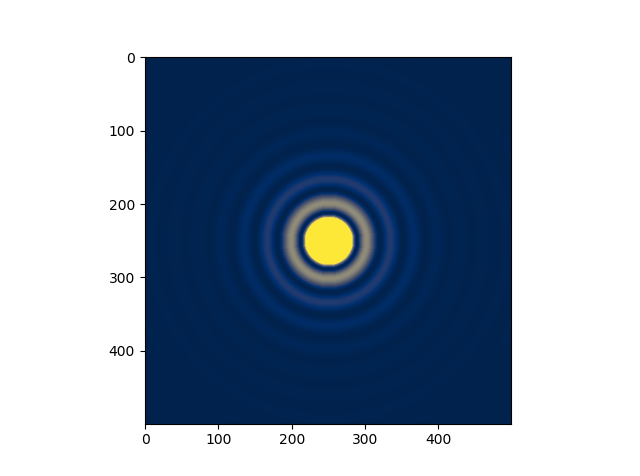
\includegraphics[width=0.7\linewidth]{DiffractionPattern}
	\caption{OUTPUT of Listing \ref{lst:L6}}
	\label{fig:diffractionpattern}
\end{figure}
\subsection{Errors on Integrals}
The numerical integrals mentioned before were only approximations. Therefore, we are able to derive their approximation errors to get an idea of the precision involved.\\

We define $x_{k}=a+kh$, a point to evaluate $f(x)$ at. Now Taylor expansion at $x_{k-1} $is given by:
\[ f(x)= f(x_{k-1})+(x-x_{k-1})f^{'}(x_{k-1})+\dfrac{1}{2!}(x-x_{k-1})^{2}f^{"}(x_{k-1}) + ... \]
\par Integrating $f(x)$ in range $[x_{k-1},x_{k}]$ gives:
\[ \int_{x_{k-1}}^{x_{k}}f(x)\cdot dx = f(x_{k-1})\int_{x_{k-1}}^{x_{k}}dx + f^{'}(x_{k-1})\int_{x_{k-1}}^{x_{k}}(x-x_{k-1})\cdot dx +\dfrac{f^{"}(x_{k-1})}{2}\int_{x_{k-1}}^{x_{k}}(x-x_{k-1})^{2}\cdot dx + ....
\]
\par Substituting $u=x-x_{k-1}$ :
\[ \begin{split}
\int_{x_{k-1}}^{x_k} f(x)\cdot dx&=f(x_{k-1})\int_{0}^{h}du+f^{'}(x_{k-1})\int_{0}^{h}u\cdot du + \dfrac{f^{"}(x_{k-1})}{2}\int_{0}^{h}u^{2}\cdot du+ ....\\
&=hf(x_{k-1})+\dfrac{h^{2}}{2}f^{'}(x_{k-1})+\dfrac{h^{3}}{6}f^{"}(x_{k-1})+O(h^{4})\\
\end{split} \]
\par where,  $O(h^{4})$ denotes the rest of the terms in the series, those in $h^{4}$ and higher.\\
\par We can do similar expansion around $x=x_{k}$ and again integrate within the given range. Taking the average of the integrals in range $[x_{k-1},x_{k}]$ with Taylor expansions at both $x_{k-1} and x_{k}$ gives us:
\[\int_{x_{k-1}}^{x_{k}}f(x)\cdot dx = \dfrac{h}{2}[f(x_{k-1})+f(x_k)]+\dfrac{h^2}{4}[f^{'}(x_{k-1})-f^{'}(x_k)]+\dfrac{h^3}{12}[f^{"}(x_{k-1})+f^{"}(x_k)]+O(h^4)
\]
\par Finally, we sum this expression over all slices $k$ to get the full integral that we want:
\[\begin{split}
\int_{a}^{b}f(x)\cdot dx& =\sum_{k=1}^{N}\int_{x_{k-1}}^{x_{k}}f(x)dx\\
&=\dfrac{h}{2}\sum_{k=1}^{N}[f(x_{k-1})+f(x_{k})]+\dfrac{h^{2}}{4}[f^{'}(a)-f^{'}(b)]+\dfrac{h^{3}}{12}\sum_{k=1}^{N}[f^{"}(x_{k-1})+f^{"}(x_{k})]+O(h^{4})\\
\end{split}
\]
\par Making the changes necessary to fit the above equation to the \textbf{Trapezoidal Rule} we have:
\[\int_{a}^{b}f(x)\cdot dx = \dfrac{h}{2}\sum_{k=1}^{N}[f(x_{k-1})+f(x_{k})]+\dfrac{h^{2}}{12}[f^{'}(a)-f^{'}(b)] +O(h^{4})
\]
Thus, to leading order in h, the value of the terms dropped when we use the trapezoidal rule, which equals the approximation error $\epsilon$ on the integral is:
\[ \epsilon=\dfrac{h^{2}}{12}[f^{'}(a)-f^{'}(b)]\]
This is the \textit{Euler-Maclaurin formula} for the error on the trapezoidal rule. Similar operations for the \textbf{Simpson's Rule} yield:
\[ \epsilon=\dfrac{h^{4}}{90}[f^{\prime\prime\prime}(a)-f^{\prime\prime\prime}(b)] \]
For programming purposes, we use the numerical approach of calculating $\epsilon$ which is given as follows:
\[\begin{split}
\textbf{Trapezoidal Rule }&: \epsilon=\dfrac{1}{3}[I_{2}-I_{1}] \\
\textbf{Simpson's Rule }&: \epsilon=\dfrac{1}{15}[I_{2}-I_{1}]
 \end{split}
 \]

\subsection{Adaptive Integral Method}
\label{subsec:3.4}
This method utilises the numerical approach of calculating the errors. We begin by calculating an approximate integral $I_{1}$ with $N$ steps. Similarly $I_{2}$ is calculated with $2N$ steps. Then, the error will be given by:$$\epsilon=\dfrac{1}{3}[I_{2}-I_{1}]$$ Furthermore, If $\epsilon>\epsilon_{0}$, where $\epsilon_{0}$ is the degree of accuracy, we double the number of steps until $\epsilon<\epsilon_{0}$. This is implemented for the \textbf{Trapezoidal Rule} as follows:
\begin{lstlisting}[language=Python, caption=Adaptive Rule, frame=single, label={lst:L7} ]
def f(x):
	return #Function here
a= #Start Range
b= #End Range
thresh= #threshold
error=1 #Seed Error
N=1 #Repetitions
I1=(f(a)+f(b))/2
while error>thresh:
	N=2*N
	h=(b-a)/N
	s=1/2*(f(a)+f(b))
	for i in range(1,N):
		s+=f(a+i*h)
	I2=h*s
	error=abs(1/3*(I2-I1))
	I1=I2
print(f'The value of integral is {I1} with error {error}')
\end{lstlisting}
\newpage
\subsection{Romberg Integration}
The \textbf{Romberg Integration Formula} is :
\[R_{i,m+1} = R_{i,m} + \dfrac{1}{4^{m}-1}(R_{i,m}-R_{i-1,m}) 
\]
which is accurate to order $h^{2m+1}$ with an error of order $h^{2m+2}$. The procedure is given as follows:
\begin{enumerate}
	\item Calculate first two estimates using \textbf{Trapezoidal Rule} :\\
	 $I_{1}\equiv R_{1,1}$ and $I_{2}\equiv R_{2,1}$
	 \item From these two, calculate the more accurate estimate: $R_{2,2}$
	 \item Thus. for each estimate we also calculate the error to meet some desired accuracy.
	
\end{enumerate}
\begin{center}


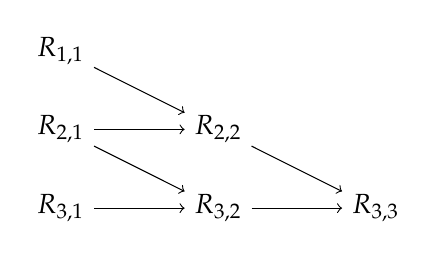
\begin{tikzpicture}[node distance=2cm][H]
% nodes

\node (A) at (0, 0) {$R_{1,1}$};
\node (B) at (0,-1 ) {$R_{2,1}$};
\node (C) at (2,-1 ) {$R_{2,2}$};
\node (D) at (0,-2 ) {$R_{3,1}$};
\node (E) at (2,-2 ) {$R_{3,2}$};
\node (F) at (4,-2 ) {$R_{3,3}$};

% arrows
\draw [->] (A)--(C);
\draw [->] (C)--(F);
\draw [->] (B)--(C);
\draw [->] (B)--(E);
\draw [->] (D)--(E);
\draw [->] (E)--(F);
\end{tikzpicture}
\end{center}

\subsection{Gaussian Quadrature}
Until now, we had been using numerical methods that had evenly spaced point within the range. However, for functions with high variation in slope, we require higher number of points of evaluation in regions of higher variations of slope. Conversely, we do not require a lot of points for functions with lesser variation in slope. This dilemma is partly solved by the \textbf{Gaussian Quadrature} method.
\par
To calculate an approximation to our integral, we have:
\[\begin{split}
\int_{a}^{b}f(x)dx&\approx \int_{a}^{b}\Phi(x)dx=\int_{a}^{b}\sum_{k=1}^{N}f(x_{k})\phi_{k}(x)dx\\
&=\sum_{k=1}^{N}f(x_{k})\int_{a}^{b}\phi_{k}(x)dx
\end{split}\]
\par Thus, we have weights $w_k$ given by:
$$w_{k}=\int_{a}^{b}\phi_{k}(x)\cdot dx$$
\par Often, we are given these weights for $a=-1$ and $b=+1$. These can be mapped to our new variables by the following equations:
$$x_{k}^{\prime}=\dfrac{1}{2}(b-a)x_{k}+\dfrac{1}{2}(b+a)\\$$
$$w_{k}^{\prime}=\dfrac{1}{2}(b-a)w_{k}$$
\subsubsection{Sample Points}
The sample points $x_{k}$ should be chosen to coincide with the zeros of the $N^{th}$ \textbf{Legendre Polynomial} $P_{N}(x)$, rescaled if necessary. The corresponding weights $w_{k}$ are:$$w_{k}=\left[\dfrac{2}{(1-x^{2})}\left(\dfrac{dP_{N}}{dx}\right)^{-2}\right]_{x=x_{k}}$$
To obtain such points, I shall use the python program discussed in Appendix.
\subsubsection{Gaussian Quadrature Implementation}
\begin{lstlisting}[language=Python, caption=Gaussian Quadrature, frame=single, label={lst:L8} ]
from gaussxw import gaussxwab #to obtain sample points and weights
def f(x):
	return #function here
a= #Start Range
b= #End Range
N= #Iterations
x,w=gaussxwab(N,a,b)
integ=0
for i in range(N):
	integ+=f(x[i])*w[i]
print(integ)
\end{lstlisting}
\subsubsection{Heat Capacity Of A Solid}
\medskip
\begin{displaymath}
C_V = 9V\rho k_B \biggl( {T\over\theta_D} \biggr)^3 \int_0^{\theta_D/T}
{ \dfrac{x^{4}e^x}{(e^x-1)^2} dx}
\end{displaymath}
\\
\begin{lstlisting}[language=Python, caption=Heat Capacity, frame=single, label={lst:L9} ]
V=10**(-3)
ndensity=6.022*10**28
debyetemp=428
N=50
k=1.38065852*10**(-23)
x,w=gaussxw(N)
def f(x):
	return (x**4)*(np.exp(x))/(np.exp(x)-1)**2
def cv(T):
	a=0
	b=debyetemp/T
	integ=0
	wk=(b-a)/2*w
	xk=(b-a)/2*x+(b+a)/2
	for i in range(N):
		integ+=f(xk[i])*wk[i]
	return 9*V*ndensity*k*((T/debyetemp)**3)*integ
T=np.arange(5,501)
C_val=[]
for i in range(len(T)):
	C_val.append(cv(T[i]))
plt.figure(figsize=(10,5))
plt.plot(T,C_val)
plt.xlabel('Temp, K')
plt.ylabel('C_V')
plt.title('Heat Capacity Of Solid Al v/s Temp')
\end{lstlisting}
\newpage
\begin{figure}[H]
	\centering
	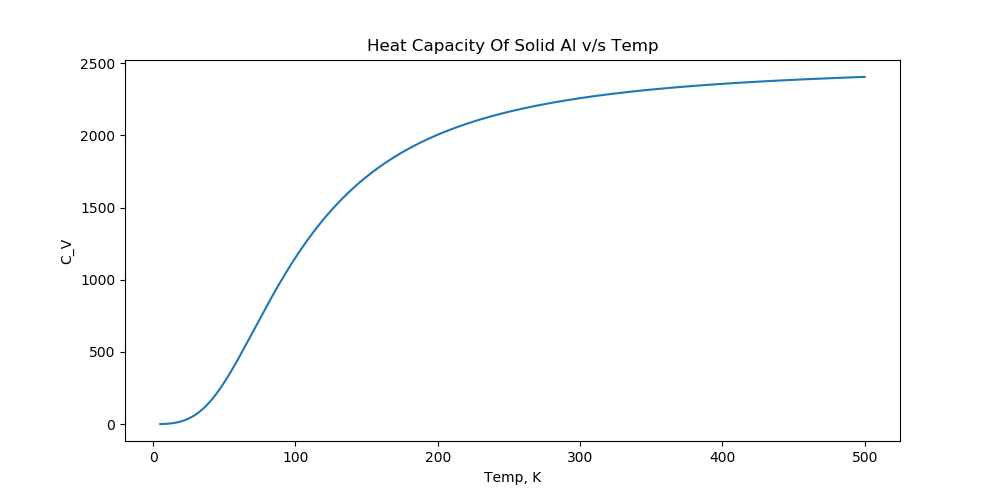
\includegraphics[width=1\linewidth]{heatcapacity}
	\caption{OUTPUT for Listing \ref{lst:L9}}
	\label{fig:heatcapacity}
\end{figure}
\subsection{Integrals over Infinite Ranges}
We cannot possibly converge on an acceptable solution for integrals with infinite ranges by a numerical approach, since there are infinite slices. Therefore, what we require is a \textbf{change of variables}. To evaluate $\int_{0}^{\infty}f(x)dx$, we substitute $$z=\dfrac{x}{1+x}$$ Then, $$dx=\dfrac{dz}{(1-z)^{2}}$$ and $$\int_{0}^{\infty}f(x)dx=\int_{0}^{1}\dfrac{1}{(1-z)^{2}}f\left(\dfrac{z}{1-z}\right)dz$$
\par Similar substitution for ranges like $(-\infty,0)$,$(a,\infty)$ etc. can be made. To evaluate in range $(-\infty,\infty)$, we divide the range at 0 and evaluate accordingly.

\subsection{Multiple Integrals}
To evaluate $$I= \int_{0}^{1}\int_{0}^{1}f(x,y)dx dy$$ We can re-write this by defining a function $F(y)$, thus $$F(y)=\int_{0}^{1}f(x,y)dx$$ Then, $$I=\int_{0}^{1}F(y)dy$$
\par Similarly, for using the \textbf{Gaussian Quadrature}, we have the \textbf{\textit{Gauss-Legendre product formula}}:
$$I\approx\sum_{i=1}^{N}\sum_{j=1}^{N}w_{i}w_{j}f(x_{i},y_{j})$$
\begin{figure}[H]
	\centering
	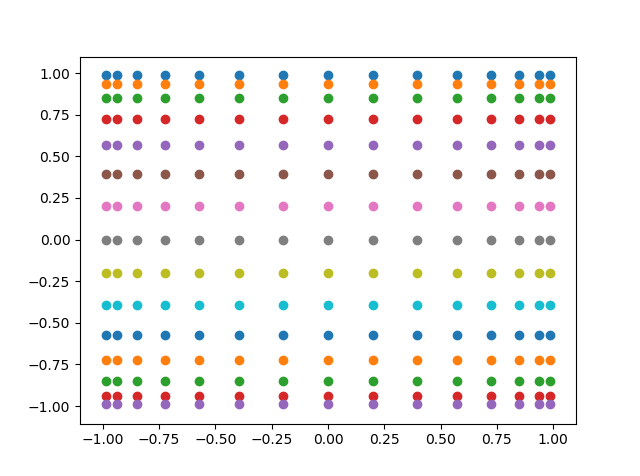
\includegraphics[width=0.7\linewidth]{multiplepoints}
	\caption{Points of Evaluation for Gaussian Quadrature}
	\label{fig:multiplepoints}
\end{figure}











\newpage
%\section{Derivatives}

\newpage
\appendix


\section{Updated Plan Of Action}
\documentclass[11pt,a4paper,leqno]{article}
\usepackage[width=15.00cm, height=27.00cm]{geometry}
\usepackage{authblk}
%opening
\title{\textbf{\huge Computational Physics}}

\author[1]{ Vinit P. Doke}
\affil[1]{{
		Department of Physics\\ 
		Indian Institute of Technology\\
		Powai, Mumbai 400076 \\
		{Email:} \texttt{vinitdoke@gmail.com , 190260018@iitb.ac.in
		}.}
}
\date{{ Mentor: Chaitanya Kumar }}



\begin{document}

\maketitle
\section{{\textbf{{\LARGE         Plan Of Action}}}}

	
\subsection{Objective}
 {\large The objective of this endeavour is to get an idea of the roll of Computation in solving Physics problems. Computational Physics complements the areas of theory and experimentation in traditional scientific investigation. Final goal would be to apply the techniques to predict outcome by simulation of the physical phenomenon.
 	
\subsection{Resources}
{\large 
\begin{itemize}
	\item \textbf{Computational Physics: Problem Solving with Computers} [RUBIN H. LANDAU]
	\item \textbf{Computational Physics} [MARK NEWMAN]
	\item \textbf{www.w3schools.com} [for learning Python]
\end{itemize}}
\subsection{General Path to be followed :}
\begin{enumerate}
	\item Learning coding in Python.
	\item Learning the necessary libraries in Python:
	\subitem NumPy
	\subitem SciPy
	\subitem Pandas
	\subitem Matplotlib
	\item Implementing Math through code:
	\subitem Integrals and Derivatives
	\subitem Solving Linear and Non-Linear Equations
	\subitem ODEs and PDEs
	\subitem etc.
	\item Monte-Carlo Simulations
	\item Application of the techniques learned so far
\end{enumerate}





\end{document}

\newpage
%input{MidTermReport}

\end{document}
